\documentclass{report}

\usepackage[latin1]{inputenc}
\usepackage[english]{babel}
\usepackage{lastpage}
%\usepackage{fullpage}
\usepackage{fancyhdr}
\pagestyle{fancy}

\setlength{\parindent}{0pt}
\setlength{\parskip}{1.8ex plus 0.5ex minus 0.2ex}
\newcommand{\class}[1]{\textsf{#1}}

\title{Map of Denmark\\
\normalsize{\textit{First-Year Project, Bachelor in Software Development, \\IT
Univ. of Copenhagen}}}
\author{
Group 12\\
Jakob Melnyk jmel@itu.dk\\
Niklas Hansen nikl@itu.dk\\
Emil Juul Jacobsen ejuu@itu.dk\\
Jens Dahl M�llerh�j jdmo@itu.dk\\
\\
Supervisors: Lars Birkedal\\
Advisors: Jonas Brabrand
Jensen and Filip Sieczkowski
}
\date{May 25th, 2011}

\begin{document}
\maketitle
\tableofcontents
\pagebreak
\chapter{Preface}
\chapter{Background}
\label{BG}
\section{Problem area}
\label{BG-PR}
Over the last decade people have switched from traditional roadmaps 
to using the web-maps. This is a change without any negative side-effects. 
The online services remove all the problems with determining the quickest 
route between two points and you spend no time browsing the pages of 
the map to find what you need. With the popular smartphones the online 
map is even more useful, since you no longer need to prepare your trip 
before you leave.

The online maps have now been used for many years and haven`t been slow 
at adopting new features to improve their usability. They have both 
implemented satellite-maps that allow us to browse the entire planet 
from above, and lately the feature called Google Street View has upped 
the stakes when allowing us to look at any direction from a given point 
of a road. The two maps that we use the most are Google Maps and the 
Danish map called Krak. These maps both have the mentioned features 
but slight differences in the way the user navigates and searches 
for routes.

Because of the widespread knowledge of the online maps, the users 
have been accustomed to certain features and ways of using the map. 
It is very important that we, with a new map program, use this knowledge 
to our advantage and don`t try to reinvent the wheel. By using some 
of the commonly used controls in our map, a user will be able to quickly 
adapt to our program and use it efficiently. 

\section{Requirements for the map}
\label{BG-R}
Our teachers had a few requirements for features in the project. The requirements were presented to us during development, in 3 steps. This made
it easier for us to focus on getting the basic features of the program to work,
but it made it harder for us to plan ahead as well.

Here is a list of the features we had to implement: 
\begin{itemize}
  \item We had to make a visual representation of all the roads from the
  dataset.
  \item We had to draw different roads in different colors.
  \item We had to adjust our drawing of the roads to the windows size of our
  GUI.
  \item We had to make mouse zooming possible.  The user should be able to drag
  the mouse from one corner of the map to another, in order to zoom in on the
  selected area.
  \item We had to implement a method to find a route from one road in the map to
  another, and we had to allow the user to find that route by clicking at each
  of the roads.
\end{itemize}
We had to consider these requirements while
deciding how the program should be designed. Of course, some of the
requirements were so self explanatory that we would have made them regardless
of them being required.
\section{Our requirements}
In the process of designing the program we made some requirements that we
wanted to make sure was met before making more advanced features. Since it was
required to make the user able to zoom-in on the map, we found it logical to
allow him or her to:
\begin{itemize}
  \item Zoom out
  \item Scroll the map
\end{itemize}
With these basic features covered, we decided which advanced featured we wanted
implement. In order to give the user a chance to find more specific places, we
decided to show the user the name of the road closest to the cursor. This means
that the user can get orientated without clicking or pressing any button. 

The most interesting feature of our \class{Map of Denmark} is perhaps the
option of selecting whether you want to travel by car or by bicycle. Many Danish
people use bicycles to travel and as such this feature is a very relevant and
nice one to have in the software. It is a feature not usually seen on
international maps - this is most likely due to the size of these maps.

We also decided to let the user create routes with an unlimited amount of
waypoints. This makes our map well suited for planning bicycling trips or longer
car rides where you want to reach more than one destination. Because this
feature can be quite demanding when a lot of waypoints are selected, we had to
make sure that the algorithm for finding routes was fast enough so we avoided
making use of the map cumbersome for an end-user.

We wanted to make sure that the shape of Denmark is recognizable when
the user has zoomed out to show the entire country. There is a balance between
showing a big amount of roads and the delay when navigating. We wanted to make
the user able to navigate the map with a reasonable amount of delay. 

The fact that we chose specific requirements for our program gave us two big
advantages. It both made the planning process easier, and it made the
structuring of the code easier to choose. In the process of creating the
program, we had to change and create new requirements for ourselves, when we
felt some feature was necessary for the end-user to have. In the last part of
the coding process, we decided on our final requirements and worked towards completing them. 
\section{Data set}
\label{BG-DS}
We have been provided with a dataset of roads and intersections in Denmark 
from Krak. Additionally we got some code for loading the data in from the 
text files. We have only made minor changes to the code for loading the data.
\subsection{UTM-coordinates}
\label{BG-DS-UTM}
It is important to note that the KrakNodes are in UTM-32 coordinates. When 
using the UTM standard the origo is placed at the south-west corner. These 
coordinates need some conversion when using in Java since the origo is placed 
differently.
\subsection{Graph}
\label{BG-DS-G}
When the data has been loaded it is stored as a Graph containing KrakNodes 
and KrakEdges. The KrakEdges are the road segments and contains the name 
of the road, an estimated drive time, a direction of traffic and references 
to the two KrakNodes that are at either end of the road.  The KrakNode itself 
contains only the coordinates for the point.
The Graph itself contains a number of useful methods for searching the data 
like getting all edges that is connected to a KrakNode. We will be using these 
methods extensively throughout the project both for drawing the map and for 
finding the route between two points.
\section{MVC structure}
\label{BG-MVC}
In order to achieve a decent code structure and separation of responsibilities, 
we utilize the Model-View-Controller (MVC) architecture. By doing this, we split 
the code into smaller sections, which can be easier to handle and easier to 
coorporate on the code.

This is because we split the code into three parts: graphical user interface 
(``view''), data handling (``model'') 'and the connection between the two 
(``controller''). Read more in section \ref{UML-MVC} on page \pageref{UML-MVC}.

\subsection{What is it? How does it work?}
In order to achieve a decent code structure, it is important to split the 
responsibilities of the program into different pieces, which work together 
to make the program work as intended.

One way to do this, is to have the graphical user interface in a class of its
own, and the rest of the program in another class. The downside to this
approach, is that it can get ambiguously where to put specific pieces of code
(button listeners and such).

We chose to utilize the Model-View-Controller (MVC) architecture, which is
another way of structuring a program (a better one). With MVC we divide our code
in three main parts, in order to achieve a decent separation of data, logic and
the graphical interface.

\begin{figure}[h!]
\centering
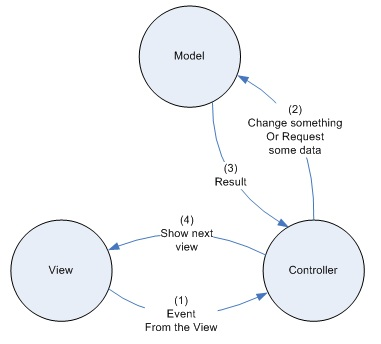
\includegraphics[width=0.5\linewidth]{images/mvc}
\caption{Overview of MVC}
\label{mvc-overview}
\end{figure}

Like the picture above shows, every graphical window has its own class. These
classes are called ``views''. Where we beforehand had one class to handle both
communication with the data and the graphical windows, we now split this into
two: ``models'' and ``controllers''.

The models handle all communication with the data sources, and every model
handle one data source. If we were to use relational databases, we would have a
model for each table in the database. In our case we only have one data source
(Krak's dataset), and therefore only have one model, to communicate with this.

Controllers
Now we only need a way to connect the graphical interface with the data. This is
where controllers enter the picture. In MVC you have one controller per view.
This controller provides the view with all the neccessary data from the models.
The controllers also have listeners on the view, that listens to events on the
view (like when the user presses a button, clicks his/her mouse and such). Then
the controller can provide new data to the view or save new data from the view
to the data source (through the models).

An example of this could be that the user updates some info and presses the 
``Save''-button. Then the controller listens to this event, passes the new data
to the models and it gets saved.
In our case we have listeners to (among other things) mouseclicks, so we can
place pins when the user clicks the map.
\chapter{User Interface analysis}
\label{UIA}
In this chapter we describe our decisions and present our analysis and
arguments regarding possible features that we find might have been interesting
to have implemented in our \class{Map Of Denmark} program.

\section{User interface as a whole}
\label{UIA-UIW}
When we designed the first version of the graphical user interface in the first
part of the project, we decided to make a window inside of the graphical user
interface where the actual map should be displayed. We chose to have this
window placed on the right side of our graphical user interface and interaction
with the user mainly placed on the left.

We believe that this is a simple way of representing a user interface for a map.
A lot of software use a menu bar with dropdown menus for selecting different
functions. When we designed our outline for the graphical user interface, we did
not design it with a huge amount of functions in mind. 

The features that we have implemented in this version can easily fit in our
simple user interface, but if features like searching for roads or other
features are included, then space and overview may become an issue on the left side.

If new features are included, we feel it would be beneficial to let the main
window change when different feature types are selected.

Below is a screenshot of our user interface. How to use it will be
explained in the \class{\nameref{MAN}} on page \pageref{MAN}.

\begin{figure}[!ht]
\centering
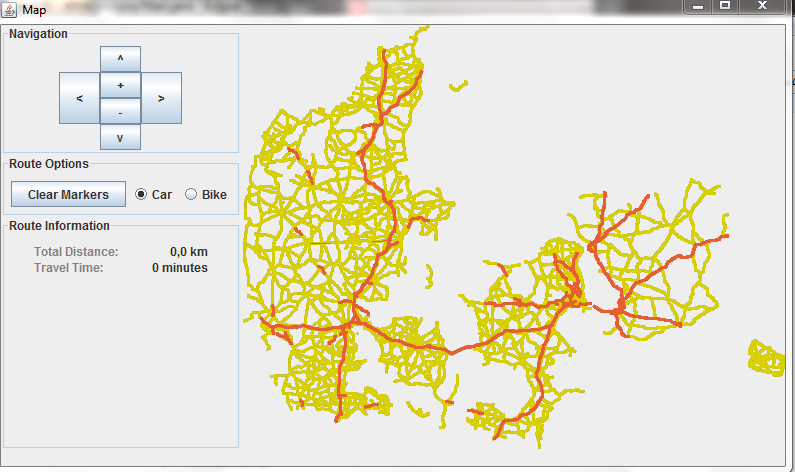
\includegraphics[width=1\linewidth]{images/PictureOfUI}
\caption{Screenshot of GUI}
\label{UIA-UIW-PIC}
\end{figure}

\section{Interesting features}
\label{UIA-IF}
This section presents some of the interesting features we have implemented.
\subsection{Zoom}
\label{UIA-IF-Z}
We have a few options for zooming in and out on the map. As described in
section \ref{BG-R} \class{\nameref{BG-R}} on page \pageref{BG-R}, it
was required that we made it possible to zoom by dragging a box around the part 
of the map the user wants to look closer at.

In addition to the option of using the mouse to zoom, we have implemented a
zoom-in and out function on the GUI and a hotkey for zooming out to the original
zoom level. We made the original zoom function a hotkey only because we did not
want to have too many buttons on the left side. We considered making it a menu bar
item, but we did not manage to get it into this version.

We felt we really needed a zoom out function, so users do not need to close the
program and start it again, when the user wants to view the map further zoomed
out. A combination of the zoom in and out functions helps the user a lot when
navigating the map.

We have limited how far a user can zoom in and out. If the user tries to zoom
out further than the original zoom level, the view will default to the original
zoom level. If the user attempts to zoom in further than a width or height of
200 in UTM32-coordinates, the zoom function will do nothing. This could 
probably be improved by zooming in on the smallest possible area at the 
position the user selected, instead of doing nothing.

\subsection{Navigation}
\label{UIA-IF-N}
We have made it possible for the user to navigate the map by using the arrow
buttons on the graphical user interface. When one of the buttons are pressed,
the ``view'' will move in the direction specified by the button. While it was
not specified as a requirement for the project, we felt it was a necessity to
implement at least basic navigation functionality.

Like we did with the two zoom functionalities, we have limited how far a user
can move around the map. The user is free to move around the map, but if user
moves outside the bounds of the map in a way where the view would show an image
that is not part of the map, the move function will not do anything.

\subsection{Hotkeys}
\label{UIA-IF-H}
We have implemented hotkeys for all the buttons on the graphical user interface
plus an additional for zooming back to the original zoom level. When we
discussed the benefits of hotkeys, we felt it was important for experienced users of the
software should have a less cumbersome time navigating the map. 

At first we just had hotkeys for the clearing of markers (mentioned in section
\ref{UIA-IF-M}) and zooming out to the original zoom level, but we later added
the hotkeys for the rest of the functionalities. If more features are added in a
future version, it would be important for us that a hotkey were provided, if at
all possible.

\subsection{Route planning and markers}
\label{UIA-IF-M}
Part of the requirements for the project was to provide the user with a way to
get the fastest or shortest route from one point to another. We accomplish this
by putting a ``marker'' at the spot where the user clicks with the mouse. The
marker shows which number in the sequence of markers it is. This will change 
if a marker is removed. Originally we had ``pins'' instead of markers, but we 
changed it, as we felt the pins we had were a bit large.

We have made it possible to place more than the two markers the project
requirements asks for. If the user places more than two markers, the software
will find the shortest route between 1 -> 2 and 2 -> 3 and so on. This was cheap for
us to implement, and we felt it added a nice touch to our program. 

We have implemented two methods of removing pins from the map. We have assigned
a hotkey to the graphical user interface button ``Clear Markers'', which removes 
all the markers from the map. The other way of removing pins is by clicking on
them. This functionality is both intuitive and confusing at the same time. It is
intuitive to click the marker you have just placed if you want to remove it, but
it is not obvious in our interface. We believe that it is enough to have the
``clear all markers'' functionality for those who do not find it intuitive to
click markers to remove them, and for the users that do find it intuitive, we
offer them an easy way to undo a missclick.

\subsection{Bike/car}
\label{UIA-IF-BC}
Another interesting feature in our \class{Map of Denmark} project is the option
to switch between bike and car routes. The user interface will start with car
selected when the program starts.

Whenever a route is calculated, it will display the length and the estimated
travel time on the left part of the user interface. When the bike option is selected, 
it recalculates the route for a bike, without visiting highways and other roads 
that bikes cannot or are not allowed to drive on. If the user switches back to the 
car mode, it recalculates the route again, but not visiting small paths and other 
roads where a car is not allowed to drive. The estimated travel time is also 
recalculated. The user does not need to have planned a route before he/she 
changes the type of transportation.

We have implemented this to help our software target a wider group of people.
The bike/car options were a bit costly to implement, but we categorized it as a
very beneficial feature and we did not feel we could leave it out.

\section{Features not implemented}
\label{UIA-NI}
% Remove this section if it is empty of content anyway.
This section presents some of the features we have chosen not to implement.
These features are not in the final program, because we did not feel there were
compelling arguments for implementing them.

Features that we wanted to implement, but did not make it into the final version,
will be discussed in chapter \class{\nameref{PRC}} on page \pageref{PRC}.

\subsection{Choice of roads to be displayed}
\label{UIA-NI-CRD}
We chose not to implement the option of selecting which roads to be displayed.
In a sense our program already does this by showing more detail the further
zoomed in the map is. It could become very confusing if the user had the option
of selecting roads, because the graphical user interface could become very
cluttered, if all the roads were listed.

One advantage to this could be the option for the user to select which roads
should be included in the route planning - ferries, highways, bridges etc. 

\subsection{Smooth scrolling}
\label{UIA-NI-SS}
We made an attempt to let the keyboard arrows scroll smoothly over the map, but
we could not implement it to work fast enough, so the user would experience
lockups and the user interface hanging at some points. A solution to this would
be to save map at images that you can scroll across - this would be faster, but
would require more disk space. Because we store the data the way we do, which 
forces us to draw every line individually every time the user moves the viewport, 
we cannot do this fast enough.

In the end, we decided the benefit of the smooth scrolling was not big enough
for us to spend a lot of time implementing this feature. The cost of changing that  
much way we draw the roads, was simply too high compared to the benefits.

\subsection{Dynamic route finding}
\label{UIA-NI-DRF}
In the final project description, a dynamic route finding feature was
suggested. If we had implemented the suggested dynamic route finding feature, a
user would be able to mark a spot and then whenever he moused over a node on the
map, he would find the route instantly.

We considered implementing this as we thought it was a
nice feature to have, but it conflicted with the algorithm we use for
calculating the route. More about the algorithms can be read in section
\ref{IMPL-DVA} \class{\nameref{IMPL-DVA}} on page \pageref{IMPL-DVA}.

\chapter{Implementation}
\label{IMPL}
Our implementation uses the MVC structure to create a practical class design. We
have prioritized to make our design as simple and intuitive as possible. We used
object oriented principles to assure that our design has both low connection
between classes (loose coupling), and a high degree of cohesion.

By following these principles we have achieved implementation with minimal code
duplication and with good possibility for extension.

Some of the basic thoughts on our design is explained in this figure:

\begin{figure}[h!]
\centering
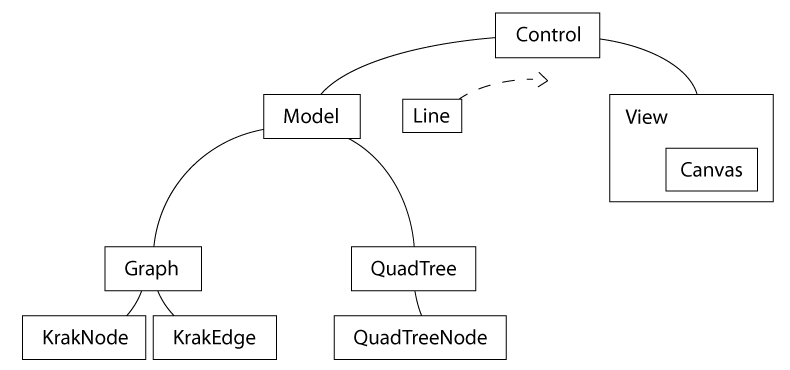
\includegraphics[width=1\linewidth]{images/BasicDesign}
\label{The basic design of our implementation. The controller gets a collection
of lines, that the view will draw.}
\end{figure}

\begin{figure}[h!]
\centering
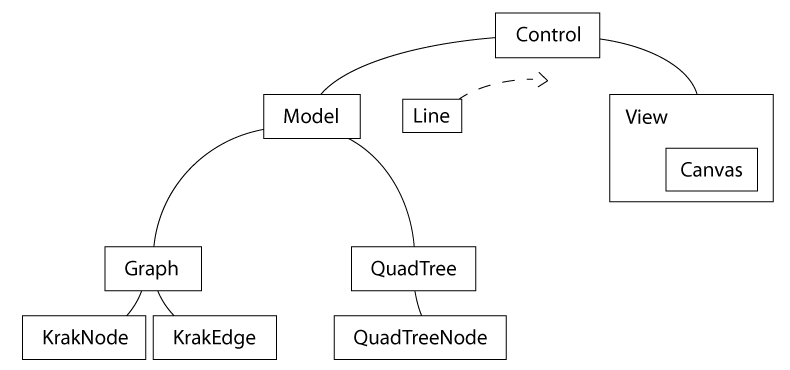
\includegraphics[width=1\linewidth]{images/BasicDesign}
\label{The pathfinding part of our implementation. The static Astar function
takes an Evaluator and a Graph and returns a path.}
\end{figure}

This rest of this chapter describes how we have implemented some of the more
interesting features of the software. We aim to describe it to enough detail that this
chapter can serve as a guideline for implementing the functionalities we
describe.

\section{UTM-conversion}
\label{IMPL-UTM}
% But what is UTM? It isn't really explained anywhere.
When the graphical user interface part of the map tries to communicate with the
model through control, some conversions of the different kind of values are
necessary. Both when going from coordinates in the java-coordinate system to
UTM32-coordinates and back.

We need to convert the values when we want to use the mousezoom and when we want
to place the markers for pathfinding. We get an input on the graphical user
interface when we mousezoom and this needs to be converted to UTM-coordinates so
that we can create the new boundaries of the zoomed rectangle.

When we place markers for pathfinding, we do the same as when we do mousezoom,
but instead we store the point as UTM32-coordinates and whenever we move the
map, we convert it back to pixel-coordinates so that we know where to draw.

The java-coordinates have origo in the top left corner with the y-coordinate
increasing the further down the y-axis you go. UTM32-coordinates are a bit
different. UTM32 has origo in the bottom left corner and the y-coordinate
increasing the further up you go on the y-axis.

% Re-phrasing needed probably.
We have a utility class with methods for converting the points back and forth.
One takes a point from the view. The model and the view itself uses this formula
for converting the pixelpoint to the UTM32-point.

Below is an illustration of the conversion from pixel to UTM.

\begin{figure}[!ht]
\centering
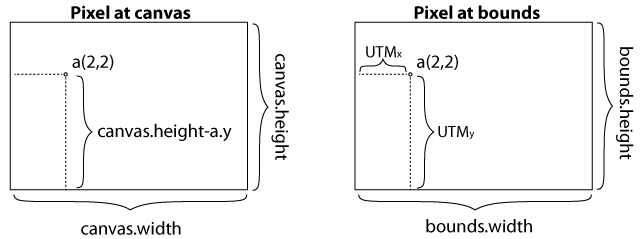
\includegraphics[width=1\linewidth]{images/UTMillu}
\caption{Illustration of UTM conversion}
\label{fig:UTMconversion}
\end{figure}

We click on a point, a, on the canvas. To calculate the the UTM coordinate
corresponding to that point, we use the formulas:

$
UTM_x = bounds_x + \cfrac{a_x}{canvas_{width}} \times bounds_{width}\\
\\
UTM_y = bounds_y + \cfrac{canvas_{height} - a_y}{canvas_{height}} \times bounds_{height}\\
\\
$

To convert from UTM to pixels we use the same formulas but reversed.

$
\\
Pixel_x = \cfrac{(a_x - bounds_x)}{bounds_{width}} \times
canvas_{width}\\
\\
Pixel_y = canvas_{height} - \cfrac{a_y - bounds_y}{bounds_{height}} \times
canvas_{height}\\
\\
$

\section{Mousezoom}
\label{IMPL-MZ}
We have implemented the mouse zoom requirement by using \class{mouseEvent}s on
our canvas. When the user presses the left mouse button down, it generates a
\class{mousePressed} event. We record the position of the mouse at the time of
the \class{mousePressed} event and wait for the \class{mouseReleased} event.
When the left mouse button is released, it generates a \class{mouseReleased}
event. We use the positions of the mouse at the \class{mouseReleased} event and
the \class{mousePressed} event to calculate new bounds for the model.

% Redundant?
As mentioned in section \ref{IMPL-UTM} \class{\nameref{IMPL-UTM}}, we use
UTM-conversion to convert pixel values into the UTM values we need.

% This paragraph can probably be longer and more detailed.
Often the user will not drag a square that is in perfect ratio with the
canvas. If it does not have the same ratio as the canvas, we change the ratio
of the dragged square behind the scenes. We do this by either adding length or
width to the dragged square. We always make sure to at least show what was
inside the box the user dragged.

If the ratio of the dragged square is smaller than the canvas ratio, we make the
dragged box wider. If the ratio of the dragged square is larger, we make the
dragged box taller.

\section{Dijkstra vs A-star}
\label{IMPL-DVA}
When planning the pathfinding feature, we had to decide between two algorithms:
Dijkstra and A*. The latter is based on Dijkstra, but achieves better performance by
using heuristics.

% First sentence should be re-phrased.
The Dijkstra algorithm uses a minimum priority queue to find the shortest path
from a given node to every other node by looking at the edges connecting nodes.
The program will take a node from the priority queue and add all the other nodes
that are connected to the current node to the priority queue. The priority queue
stores a value with the node, which is the distance to the current node
plus the length of the edge between the two. Since the priority is made to return
the node with the smallest value associated with it, the next node in line will
always be the one which is closest to the start node. This procedure continues
until all nodes have been visited and by logging what edge led to all the nodes,
it is possible to trace back the route to the start node.

This algorithm is great if we need to find the distance from one point to many other
points, but can be quite slow when using it for finding a path between to nodes,
since it just searches in all directions without thinking about in which direction the
target node is.

% ``estimated distance ... the given node'' - should be more clear.
This is where A* comes in handy. The A* algorithm is a modification of Dijkstra's
algorithm that also looks at the estimated distance from the given node when
determining the value for the priority queue. When using the geographical distance
as a measure of best route, the value would be the current distance from the start
node plus the direct distance to the target (as if there were a road directly to
the target). With this subtle change, the algorithm will prioritize nodes that are
relatively closer to the target rather than those that are in the other
direction. This makes the algorithm much faster since it will not pay much attention
to the roads that are not in the direction of the target.
We have decided to use the A* algorithm since we only calculate routes between
two distinct nodes and therefore don`t need the route from the start node to all
others. The time reduction that A* gives is also a definite plus since no user
wants to sit and wait too long for the program to find a route.

\begin{figure}[!ht]
\centering
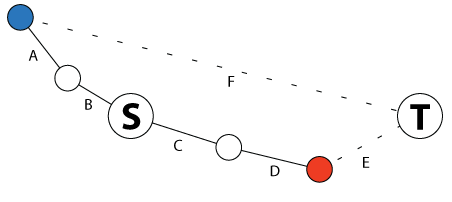
\includegraphics[width=1\linewidth]{images/AstarVSDijkstra.png}
\label{}
\caption{Astar vs. Dijkstra example. The dashed lines are the direct distances,
used by Astar. The Dijkstra algoritm will check the blue node before the red
node, because B+A < C+D. The Astar algoritm will check the red node before the
blue node, because C+D+E < B+A+F.}
\end{figure}

The smaller the difference from the direct distance is to the actual fastest
possible route, the more we will benefit from the A-star technique. This
difference will often be bigger for the routes calculated for the car. This is
because the fastest route would be a straight highway, which often is far from
possible. We can therefore conclude that the A-star technique typically is more
of a benefit when calculating routes for bicycling because they rely on the
distance.

\section{Evaluator}
\label{IMPL-EVA}
% Perhaps talk a bit more about evaluators and our default evaluators (bike and car).
In order to make our path finding algorithm flexible enough for different
interpretations of the ``best route'', we have added an entity called \class{Evaluator}.
This is an object that has the responsibility of evaluating a node relative to
the target node. The \class{Evaluator} also has the responsibility of calculating the
heuristics that the A* algorithm relies on. By using the \class{Evaluator} we are able to
use the same path finding algorithm for two very different tasks; the biking route and
the car route. The major difference between these is that the bike's heuristics is based
on the distance, where as the car's heuristics is based on the total drive time. This
implementation is also a good example of making our code ready for future features,
since if we needed to add other means of transportation or simply variations of the ones
we have, we would only need to create new \class{Evaluator}s and not change
a single line of code in the A* algorithm.

\section{Quadtree}
\label{IMPL-QT}
% Quadtree, serialization and threading should maybe be in its own section
% (called optimizations or something)
% This section reminds me of a lot of different statements, not really joined together.
% Needs more pros and cons, and should be ``longer'' / more in depth.
In order to improve the drawing of our map, we have implemented a data structure
called quadtree. The quadtree divides our map in four squares. In these four squares
it divides our roads again into smaller squares, and we keep doing this, until we reach
an amount of roads that is manageable.
When we want to retrieve data from the map, we can give the quadtree a
rectangle, and it will return all the roads within our smaller squares that intersect
that rectangle. This technique optimizes the drawing of the roads, because we
limit the amount of roads we draw.

However, when viewing the entire map of Denmark, this implementation does not help
us. Therefore, it is necessary to only to draw the bigger roads when zoomed out. We
have discussed two different techniques to do this.

The simplest solution would be to iterate over the roads returned and then
remove the road we do not want to draw. However, it would be more efficient to sort the
roads before we put them in the quadtree, and then have them sorted in the quadtree.
With this method we will not to iterate and remove the roads all the time.

\begin{figure}[h!]
\centering
\includegraphics[width=1\linewidth]{images/UnsortedQuadtree.png}
\caption{Unsorted Quadtree. A quadtree were the roads are not sorted}
\label{IMPL-USQ}
\end{figure}

We have discussed two different ways to sort the roads in the quadtree.

The first technique relied on dividing the types of roads into different quadtrees.
With this implementation, we only implement the quadtrees containing the roadtypes
we want to draw, into our drawing.

\begin{figure}[h!]
\centering
\includegraphics[width=1\linewidth]{images/MultiQuadtree.png}
\caption{Multi-quadtree. First node divides the roads into more
quadtrees.}
\label{IMPL-DCQ}
\end{figure}

The second technique relied on putting the bigger roads at the top of the
quadtree when building it. Then we could specify at which depth we wanted to
search the quadtree. We called this 'the depthcontrolled quadtree'.

\begin{figure}[h!]
\centering
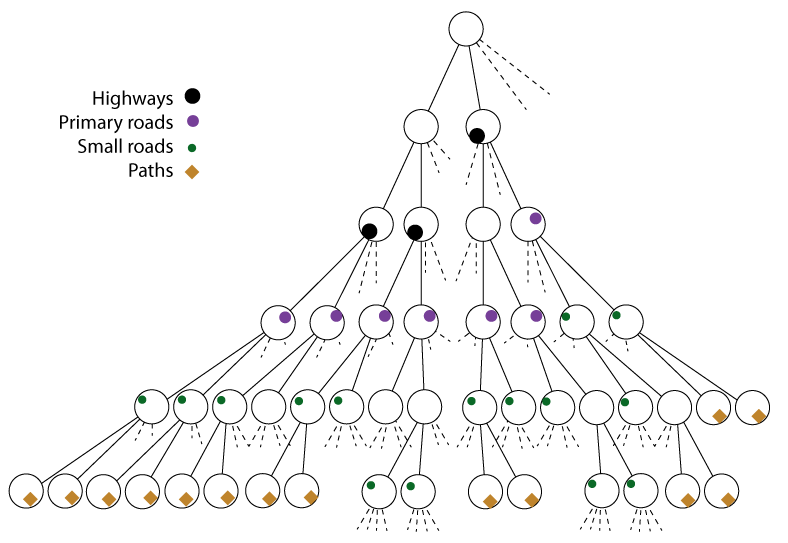
\includegraphics[width=1\linewidth]{images/DepthcontrolledQuadtree.png}
\caption{The depthcontrolled quadtree.}
\label{IMPL-DCQ}
\end{figure}

The two methods both have advantages and disadvantages.

% And how is this different to our multi-quadtree were we always use the two upper quadtrees?
The depth controlled quadtree would return more roads than the multiquadtree,
because the big roads would lie in big rectangles, and therefore be drawn more
often.

The depth controlled quadtree requires less RAM than the multiquadtree,
because it requires less instances of object QuadTreeNode.

% This is almost not measurable and the pros greatly outweighs the cons.
The multiquadtree is less efficient to search through than the
depthcontrolled quadtree, because we must run through each quadtree
individually.

Looking at the advantages and disadvantages of these quadtrees, we have chosen
to implement the multiquadtree. We have done this because it is the drawing of
the roads that slows our implementation. The efficiency of our program is not
affected by the efficiency of the quadtree searhc. The efficiency of the map is
affected because of the number of roads drawn.

\section{Serialization}
\label{IMPL-SERI}
We observed that the user had to wait quite a long time for the program to start. This
was because every time we start the program, we loop through the entire dataset given
to us by Krak. This data-set is huge, and because of this it takes quite a lot of time to
start the program. Because we need to load all these data, the user is presented with
a blank screen for a long time, before all these data are loaded and the program starts.

We started looking for a way to speed up the loading process, so the user has a map in
front of him or her quickly, when the user starts the program. What takes the most time
is looping through the data and creating the needed datastructures (quadtrees, the
graph and so on), so if we could skip these steps or speed them up, we could save a lot
of time.

This is where serialization comes into play. By serializing an object, you transform your
object into something that can be passed around, through streams and such. So by
serializing objects, you can save them to files. If the object to be serialized contains
references to other objects, these will also be serialized (if they are Serializable /
implements java.io.Serializable).

By doing this, we only need to build our datastructures the first time you start the program.
After the objects have been created, they are been serialized and saved to files. The next
time the user starts the program, we check whether the data has been changed. We check
this by checking the MD5 checksum of the file, with
\class{MD5Checksum}\footnote{We borrowed this code from \cite{MD5}} (we didn't
write this class ourselves). When we serialize the objects, we also save the checksum to a config file. If the data hasn't been changed (i.e. the checksum is the same), we load the objects that
we saved, instead of making them all over.

We serialize all the quadtrees, the graph and the maxbounds-object (specifying the bounds
of Denmark), as these are the objects we need for the program to run. When saved to the
harddrive, it is around 65MiB, which is okay, given the sizes of harddrives today.

We save all these objects to one single file, in order to keep the references. If we didn't do
this, the references will be ruined, which can break the program. We experienced problems
with this, as nodes and edges is both stored in the quadtrees and the graph. If we serialized
and saved the quadtrees in one file, and the graph in other file, a given node will be saved
twice, and when we load the data from the serialized files, the node will exist twice, and it
won't be the same node. But if we save the objects to a file through the same stream, we only
get one of each, which leads to less RAM usage, less harddrive usage, faster loadtimes and
fewer bugs.

\subsubsection{Threading}
By serializing our main objects, we cut several seconds of our load times. But we can do it
even faster. We are serializing several objects, but only few of them are needed right from
the start of the program. So what we can do to speed it up even more, is loading the few
necessary objects, and then load the rest in the background. We do this with threads.
We load the few objects we need from the start, then create a new thread to load the rest
of the objects, and in the mean time, we create the window and draw the map.

The same goes for the first run. The user doesn't need to wait for the program to finish
serializing and saving to files. By using threads, we can create the datastructures, and
then immediately show the window to the user, while saving the objects to files in the
background.

During load time (when loading from the serialized files, after the window is shown to the
user) not all quadtrees are loaded. So we did encounter a problem when querying the
quadtrees, when not all of them were loaded. We solved this by putting the querying in
a try/catch, and when a problem occurred (index out of bounds, when trying to access a
quadtree not yet loaded), we simply stopped looking through more quadtrees and just
return what we found so far. Then later on, when all quadtrees were loaded, we could
return all edges. The user wouldn't notice the lack of roads, as the user only sees a limited
amount of roads anyway.

We did encounter another problem, when trying to use the graph (for pathfinding) when the
graph wasn't done loading. We solved this by using a simple loop, that check if the graph was
set. As long is the graph wasn't available, the main thread would simply hold and wait for the
loading to finish. This is probably the only time where the user would notice that everything isn't
quite loaded, but the loading happens so fast, that it probably won't be a problem anyway.
\chapter{UML-diagrams}
\label{UML}

Figure \ref{control-flow} shows our implementation of the MVC architecture.
Because we have exactly one window, we chose to name our view and controller ``\class{View}'' and 
``\class{Control}'', respectively. The same goes for the models. We only have one data 
source (Krak's data-set), and because of that our model is called ``\class{Model}''. We could 
have named these three classes something different that may have been more meaningful 
in terms of the \class{Map of Denmark} context, but we chose these name in order to make 
our architecture clear.

We wanted to keep the models as ``trimmed'' as possible, although our
\class{Model} is quite long. But the amount of (public) methods is small, so
looking at it from outside, it is a skinny model. The reason we wanted to keep
the models skinny, is because it is not the model's responsibility to deliver
the same data in different ways, do a lot of calculations or stuff like that. It
only acts like a ``middle-man'', delivering data to other classes. If some class
wants the data in another way, they will need to convert it themselves.

\class{Control} makes sure the models and the view can understand each other. The view 
only knows about pixels, but it has no idea about UTM coordinates. The model only knows 
about UTM coordinates, but doesn't know anything about pixels. So for getting these two to 
communicate, we need to convert pixels to UTM and vice versa.

We created some helper-classes (\class{PointMethods} and \class{RectangleMethods}), 
which are located in the \class{utils} package. These take care of checking whether a point 
is within the maximal bounds of the map, converting a pixel coordinate to a UTM coordinate 
and vice versa. We did this for being able to do this in several files, without the need to have 
duplicate code. For our program right now, this isn't really a problem, as we only have one 
model, one controller and a view. But if we were to have more, we would either need to copy 
these helper-methods into the other classes (BAD), or put them in a separate class. But even 
though we only have one of each, the helper-classes are still an advantage, as
they make the code cleaner and easier to maintain and test, because we can test
these helper-classes seperately.

So in essence, we have two parts (the model and the view) that need to communicate 
somehow, in order to display the data on the screen. But they speak different languages, so 
we put in a middle-man (the controller), responsible for the communication between the two.

\section{Control flow}
\label{UML-CF}
The easiest way to understand our flow through the program and how the individual parts 
talk together, is by using an example. Let us say the user has already clicked the map and 
placed a marker. Now the user clicks on the map again to place another marker.

\begin{figure}[h!]
\centering
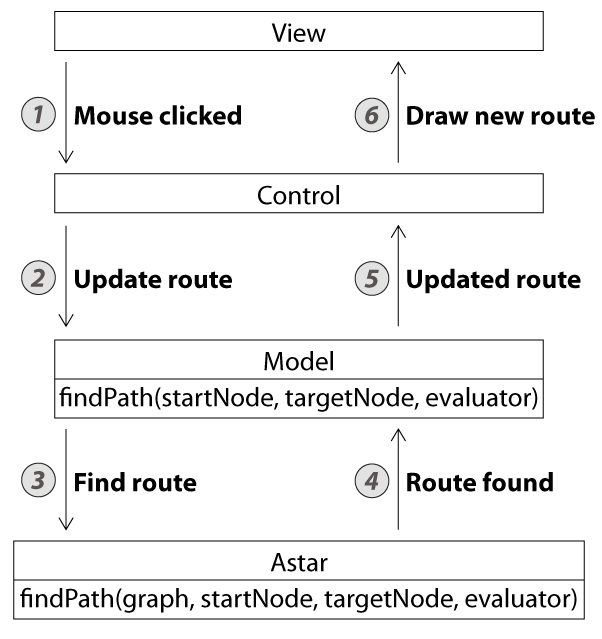
\includegraphics[width=0.75\linewidth]{images/SimpleControlFlow}
\caption{The basic control flow of our Map program}
\label{control-flow}
\end{figure}

The controller has placed listeners in the view, so when a MouseClicked event
happens, the controller is called. First it checks if there is another marker
at the spot of the click. If there is, this will be removed, and the model is
told to clear the route. If there is still over two markers placed, the model is
asked to calculate a new route.

If there isn't a pin where the user clicks, we place a new pin. If the user has placed two or 
more pins, the controller calls its own findPath-method from point 1 to point 2, point 2 to 
point 3 and so on. The findPath()-method tells the model to find a path between the two 
points given.

The model then asks a helper-class to find a path, using the A* algorithm, and provides it 
with the graph and the two points. When a path is found, it is saved in the model, ready 
for use in the controller.

The final step is getting the view to draw the route. The controller gets ready for a repaint
by fetching the route from the model. Then it passes this route to the view's repaint-method, 
and the view paints the road.
\chapter{Tests}
\label{TEST}
\section{WhiteBox: closestEdge}
\label{TEST-CE}

\section{JUnit}
\label{TEST-JU}

\section{System test}
\label{TEST-ST}
\chapter{Manual}
\label{MAN}

This manual will explain the basic use of the map, as well as its
advances features. The images are from mac osx and might look different on other
operating systems.

\section{Navigation}
\label{MAN-N}
At startup, the entire country of Denmark is shown. Now, we can move around the
map with both the diretion buttons in the top left corner, and the arrow keys.
To move west, click the button
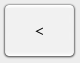
\includegraphics[height=1.3em]{images/westbutton.png} or press the left arrow
key. This goes for all 4 directions.

\begin{figure}[h!]
\centering
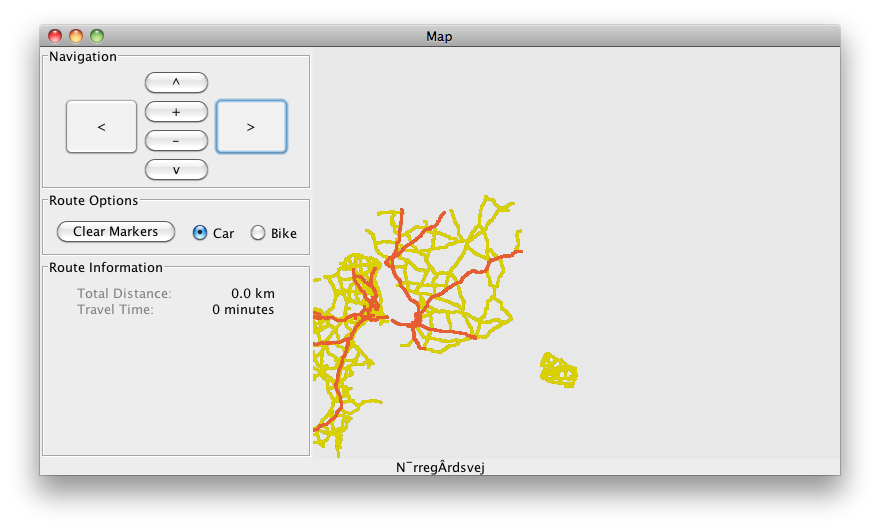
\includegraphics[width=1\linewidth]{images/man-move.png}
\caption{Zooming in on Copenhagen}
\label{MAN-Z-COP}
\end{figure}

\section{Zoom}
\label{MAN-Z}
To zoom-in on the map, click the

\includegraphics[height=1.5em]{images/zoominbutton.png} button in the navigation
panel.

To zoom-in on a specific area, click and drag a rectangle around that
area on the map. A blue transparent rectangle will show you what you have
selected. To zoom-in, release the mousebutton.

Fore example, if you want to zoom-in on Copenhagen,
click the upper left corner of the city, and drag the cursor to the lower right
corner.

\begin{figure}[h!]
\centering
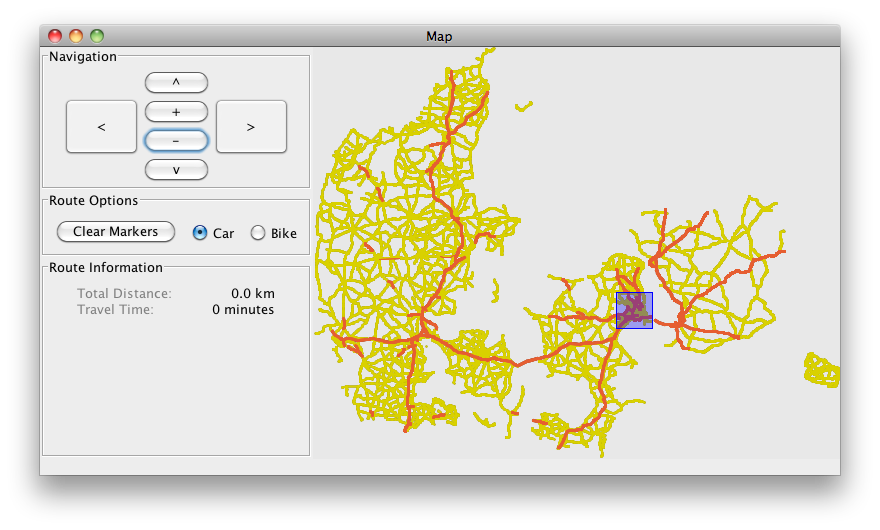
\includegraphics[width=1\linewidth]{images/man-copenhagen.png}
\caption{Zooming in on Copenhagen}
\label{MAN-Z-COP}
\end{figure}

To zoom-out of the map, click the

\includegraphics[height=1.5em]{images/zoomoutbutton.png} button. To return to
the startup view (showing the entire map of Denmark) press the esc button.

\section{Route find}
\label{MAN-RF}
To find a route from one point to another, you must specify a start and an end
location. Click anywhere on the map to choose your start location. A light blue
marker will appear, containing the number �1�. To choose your end location,
click at another location. A marker containing the number �2� will appear. The
best route from 1 to 2 will be calculated, and shown on the map as a blue path.
To extend your route with more markers, you can click at a new location on the
map. You can repeat this an unlimited amount of times. You can delete one of
your markers by clicking at its root. To delete all marker, click the button
'clear markers'.

\begin{figure}[h!]
\centering
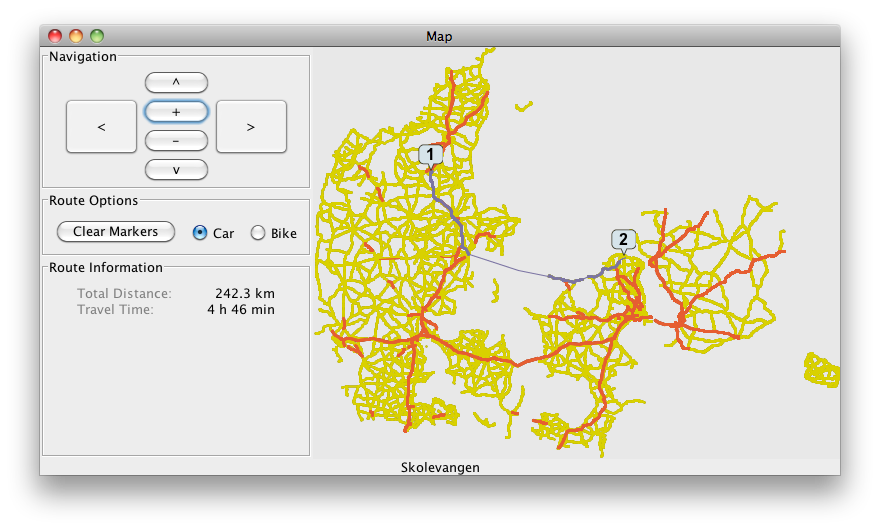
\includegraphics[width=1\linewidth]{images/man-route.png}
\caption{A route from 1 to 2 has been calculated}
\label{MAN-RF-IMG}
\end{figure}

\section{Bike/car}
\label{MAN-BC}
When calculating routes, it is important to specific which form of
transportation you wish to use. Choose your preferred style of transportation by
selecting the corresponding radio button.

\begin{figure}[h!]
\centering
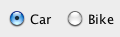
\includegraphics[height=2em]{images/radiobuttons.png}
\caption{The radiobuttons}
\label{MAN-BC-IMG}
\end{figure}

To form of transportation you use will have big insfluence on what route is
calculated. A route for a car will use highways, while a route for bicycles will
use paths.

\section{Resize}
\label{MAN-RS}
To resize the map, drag the window as you would with any other application. The
map will automatic adjust to the new size of the window.
\begin{figure}[h!]
\centering
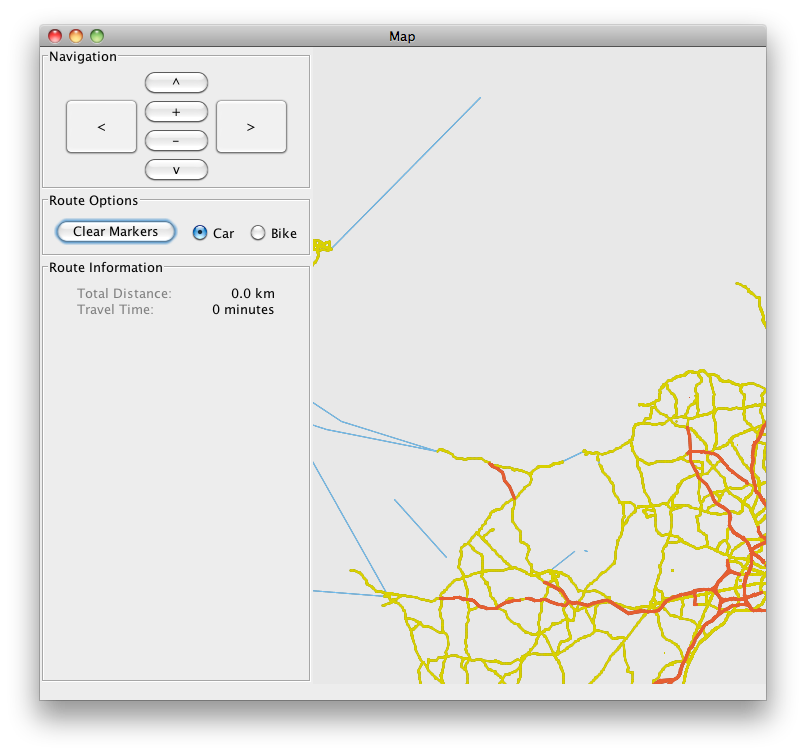
\includegraphics[width=1\linewidth]{images/man-resize.png}
\caption{The map has been resized}
\label{man-radio}
\end{figure}
\chapter{Product conclusion}
\chapter{Group norms}
\label{GN}
We wrote a constitution before the project was handed out to us. In this
constitution we describe what we require of each other and ourselves in terms of
working on the project. We felt we made some rather strict requirements so that
we were sure to get some work done. This backfired a little bit, because we were
not able to keep all of the agreements we made, but it worked for the most part.
We later changed the agreements  We later changed them a bit once our schedule
cleared up from lectures early May.

This is the requirement part of our constitution:
\begin{itemize}
  \item Check mail at least once a day
  \item Tell the rest of the group in time if you have trouble getting things done on
  time.
  \item Admit when you are not done on time.
  \item Do not waste time when we have meetings.
  \item Respect that different people work in different paces and different
  ways.
  \item We need to evaluate often.
\end{itemize}

We also tried to get a average of our level of ambition. Our goal was always to
do what we could manage to do in the time frame that we had and without wasting
time. In other words, we strived for being done early, by planning what we really 
wanted to have, and if we had time left, it was a bonus.

\section{Meetings}
\label{GN-M}
We structured our work together in ``meetings''. A meeting was whenever we were
together working on the project - these were to be done at the ITU. The
structure of a meeting was simple:
\begin{itemize}
  \item Leader of the meeting presents his plans, if any, for today. 
  \item Leader selects someone to write down what happened at the meeting.
  \item What have we done since last time?
  \item Who does what today?
  \item Work today.
  \item Fifteen minutes before work ends: decide on homework for next time and
  select leader of the next meeting.
\end{itemize}
Before our lectures ended in early May, we had meets Tuesdays and Fridays from
10 AM to 4 PM. After lectures ended, we felt only meeting Tuesdays and Fridays
would be too little time spent in meetings. So we decided to make our meetings
one and a half hours shorter, but instead meet on Mondays, Wednesdays and
Fridays from 10 AM to 2:30 PM.
\chapter{Diary}
In this project we have kept two types of diaries. One type in our meeting
documents and one in a spreadsheet. The meeting document diary was done from
meeting to meeting, so that we kept track of what everyone had done before each
meeting.

The spreadsheet diary was kept as a seperate document where we wrote down
whenever we had done something outside of meetings. 

We did not focus very much on keeping the spreadsheet up to date, because we
had the meetings (mentioned in chapter \ref{GN}), where we kept track of our
progress in the group. This made the spreadsheet sort of obsolete. We have
included it anyway though, as we feel it has been a part of the process.

Our worksheets can be found in appendix \ref{APP-WS} on page \pageref{APP-WS}.
They are written in Danish, as we had all of our meetings in Danish. The spreadsheet
diary is in appendix \ref{APP-SS} \class{\nameref{APP-SS}} on page
\pageref{APP-SS}. The spreadsheet diary is also written in Danish.
\chapter{Worksheets}
\chapter{Process description and reflection}
\end{document}